\chapter{Resultados e Discussão}\label{cap:resultados}

\section{Sequenciamento e controle de qualidade das leituras}
Após o sequenciamento das amostras, foram obtidas 7.8 milhões de leituras de tamanho médio de 
223 pares de base para a amostra ACT016 e 7.4 milhões de leituras com tamanho médio de 222 pares de base
para a amostra ACT094. Após a filtrar as leituras utilizando a ferramenta Trimmomatic, retivemos
6.2 milhões de leituras com tamanho médio 113 pares de base \(perda 21,5\%\) para ACT016 e 6.1 milhões
de leituras com tamanho médio 145 pares de base\(perda de 18,5\%\).

Baseando-se num tamanho de genoma variável de 3 a 10 milhões de bases para \textit{Rhodococcus}, podemos
determinar a cobertura real estimada pela fórmula $C= (L\cdot N)/G $ sendo $C$ a cobertura, $L$ o comprimento
médio das reads e $G$ o tamanho do genoma. A partir disso, obtivemos que a cobertura para a amostra ACT016 Após
filtrar as leituras está entre $70$ e $233,53$ vezes. 
Para a amostra ACT094, consideramos o tamanho do genoma de referência de \textit{Brevibacillus Brevis}(NZ\_LR134338) 
de 6.2 milhões de bases e estimamos a cobertura em aproximadamente $142,66$ vezes.

As qualidades médias das sequências pode ser observada a partir dos gráficos a seguir gerados pela ferramenta FASTQC:

\begin{figure}[H]
	\caption{Gráficos representando a qualidade média das leituras da amostra ACT016 na escala PHRED}
	\label{fig:fastqc_antes}
	\centering
	\begin{minipage}{.45\linewidth}
		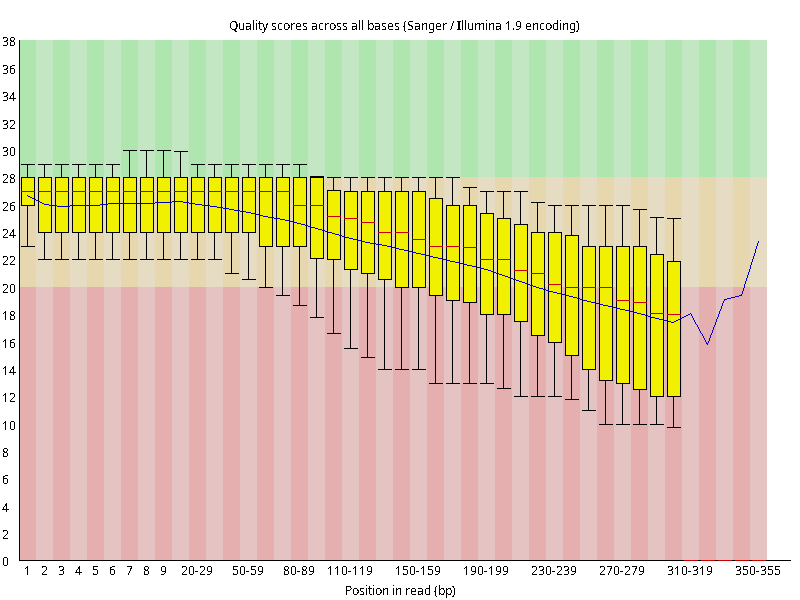
\includegraphics[height=.8\linewidth]{imagens/read\_qc/002.png}
	  \end{minipage}
	  \hspace{.05\linewidth}
	  \begin{minipage}{.45\linewidth}
		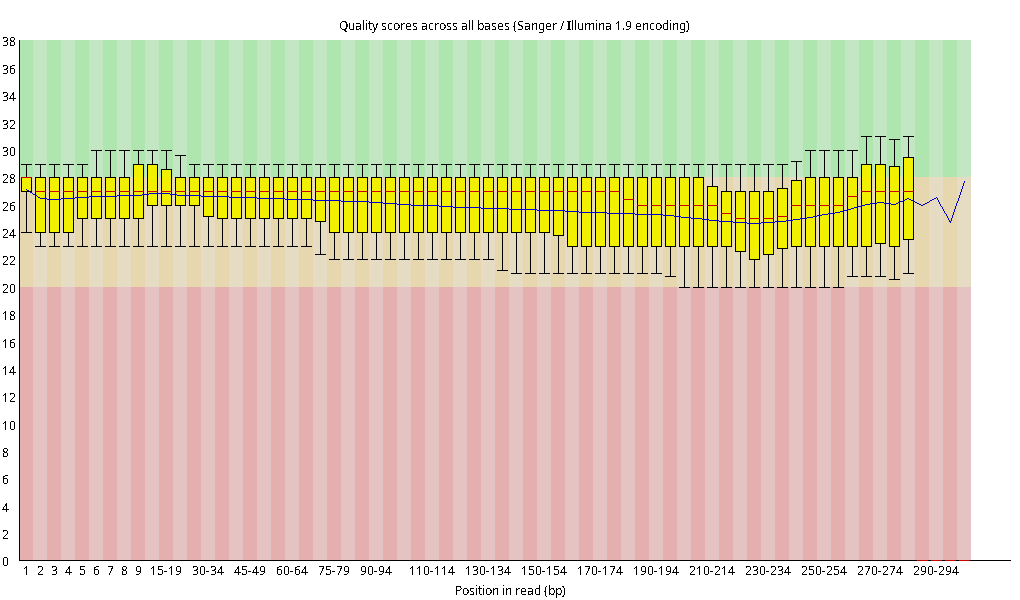
\includegraphics[height=.8\linewidth]{imagens/read\_qc/002trimmed.png}
	  \end{minipage}
    \begin{small}\textbf{Fonte: O Autor (2022)}\end{small}
\end{figure}
\vspace{\floatsep}
\begin{figure}[H]
	\caption{Gráficos representando a qualidade média das leituras da amostra ACT094 na escala PHRED}
	\label{fig:fastqc_antes}
	\centering
	\begin{minipage}{.45\linewidth}
		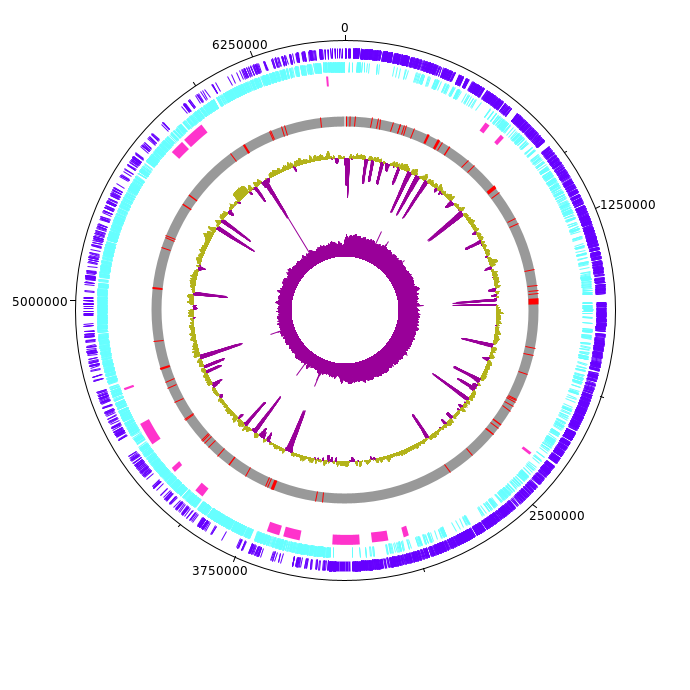
\includegraphics[height=.75\linewidth]{imagens/read\_qc/004.png}
	  \end{minipage}
	  \hspace{.01\linewidth}
	  \begin{minipage}{.45\linewidth}
		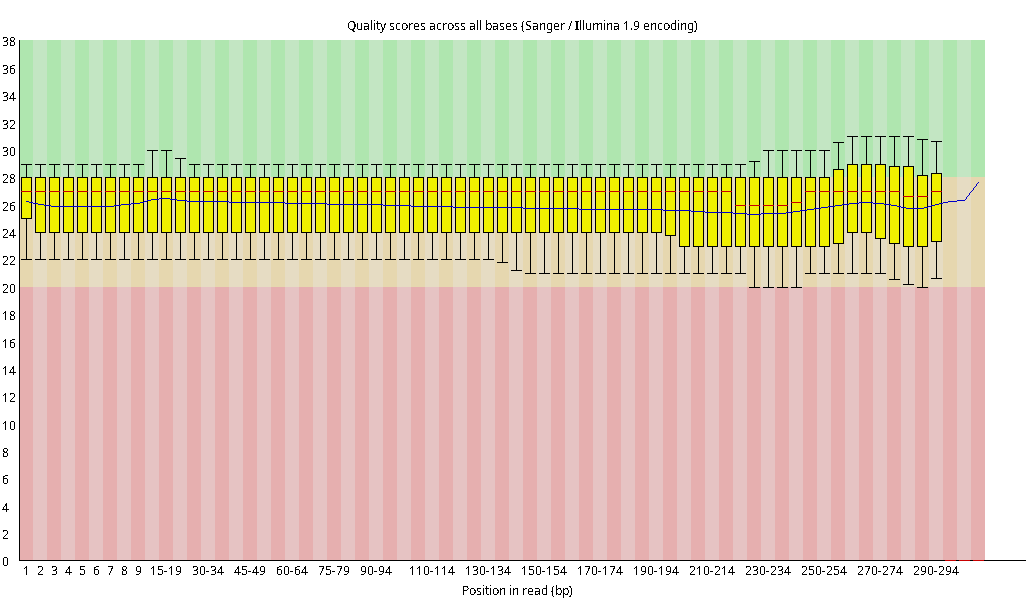
\includegraphics[height=.75\linewidth]{imagens/read\_qc/004trimmed.png}
	  \end{minipage}
    \begin{small}\textbf{Fonte: O Autor (2022)}\end{small}
\end{figure}
\vspace{\floatsep}

A partir desses gráficos podemos observar a perda de qualidade no final das leituras, um tipo de limitação
técnica comum ao utilizar sequenciadores da plataforma \textit{Illumina}, porém o término em baixa qualidade
pode ser removido após a filtração, tendo uma qualidade média ao longo da sequência próximo de PHRED 26 e
removendo sequências abaixo de PHRED 20 ( que representa probabilidade de erro maior que 1 em 100).


\section{Montagem dos genomas}

\subsection{016}
\begin{figure}[H]
	\caption{Report do software QUAST para as montagens da amostra 016}
	\label{fig:quast_16}
	\centering
		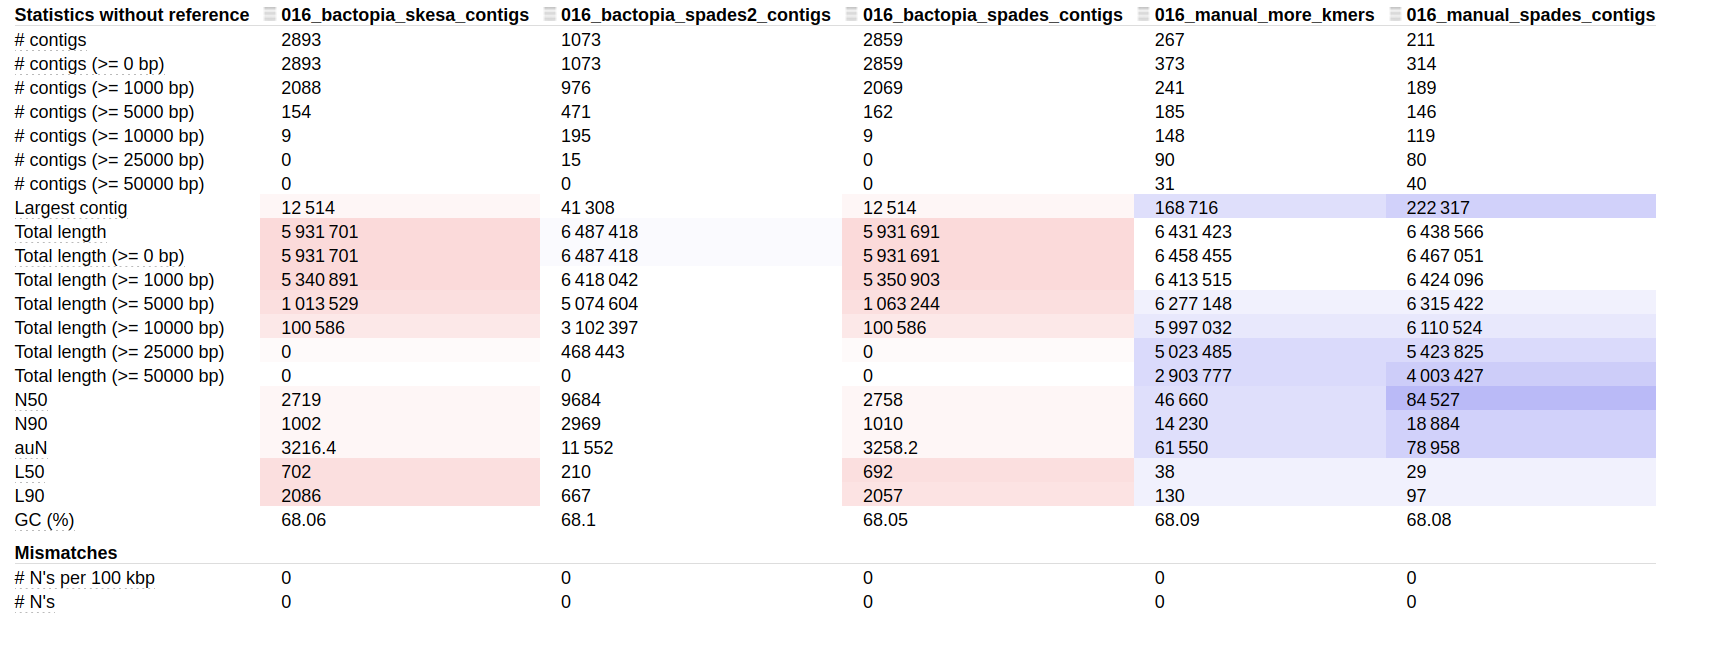
\includegraphics[height=.45\linewidth]{imagens/assembly\_qc/016assembly.png}
    \begin{small}\textbf{Fonte: O Autor (2022)}\end{small}
\end{figure}
\vspace{\floatsep}

A melhor montagem para a amostra ACT\_016 é a montagem \textit{manual_spades} que foi feita utilizando
o montador spades junto com a correção do software shovill. Essa montagem foi escolhida por ter o maior
valor de L50 (menor quantidade de contigs para atingir 50\% do número de pares de base) e maior 
\textit{contig} em tamanho absoluto ( 222 mil pares de base). O conteúdo GC de 60\% dessa montagem está de acordo
com o descrito por \citeonline{yadav2018} para Actinomicetos.

\subsection{094}

\begin{figure}[H]
	\caption{Report do software QUAST para as montagens da amostra 094}
	\label{fig:quast_16}
	\centering
		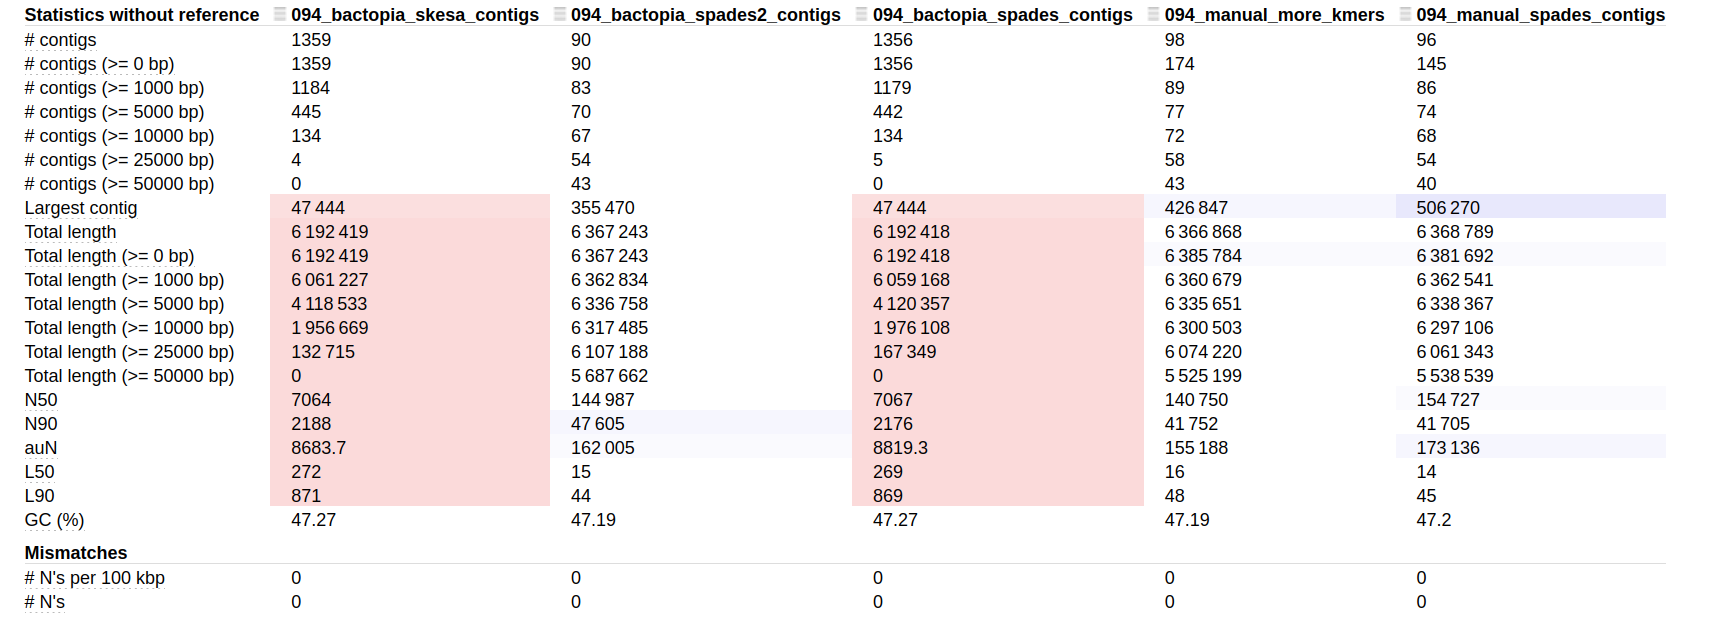
\includegraphics[height=.45\linewidth]{imagens/assembly\_qc/094assembly.png}
    \begin{small}\textbf{Fonte: O Autor (2022)}\end{small}
\end{figure}
\vspace{\floatsep}

De maneira similar, a melhor montagem para a amostra 094 também é a montagem \textit{manual_spades}.
possuindo um valor similar a montagem \textit{more_kmers} porém se diferenciando por possuir a maior \texit{contig}
com aproximadamente 80 mil pares de base a mais, um fator muito relevante para a posterior montagem do genoma completo.
O conteúdo GC também está de acordo com valores comumente encontrados em \texit{Brevibacillus brevis} \cite{nakamura1991bacillus}.

\section{Predição de espécies e pureza da montagem}
